
\chapter{Optimisation Strategy}

\section{Profitability Cost Model}\label{sec:profit-model}

After generating the code of the merged function, we need to estimate the code-size benefit of replacing the original pair of functions by the new merged function.
In order to estimate the code-size benefit, we first compute the code-size cost for each instruction in all three functions, which is done with the help of the compiler's target-specific cost model.
% The actual cost of each instruction comes from querying this compiler's built-in cost model, which provides a target-dependent cost estimation that approximates the code-size cost of an IR instruction when lowered to machine instructions.
% Our implementation makes use of the code-size costs provided by LLVM's target-transformation interface (TTI), which is widely used in the decision making of most optimisations~\cite{porpodas18b,pohl18}.


The compiler's cost model provides a target-dependent cost estimation that approximates the cost of an intermediate representation (IR) instruction when lowered to machine instructions.
Compilers usually provide a performance cost model, which estimates the latency of each instruction, and a code-size cost model, which estimates the binary size of each instruction.
These cost models play an essential role in the decision making of most compiler optimisations~\cite{porpodas18b,pohl18}.
The absolute cost estimated for one instruction is less important than its relation to the cost of other instructions.
Ultimately, these costs are used for comparing two pieces of code, informing the compiler's decision of whether or not a given transformation is profitable.
%These cost models need to be defined only once per target architecture but they play an essential role in the decision making of most compiler optimisations. 

In order to estimate code-size cost of one function, we sum up the code-size cost of all instruction by querying the cost model.
In addition to measuring the difference in size of the merged function, we also need to take into account all extra costs involved:
$(1)$ for the cases where we need to keep the original functions with a call to the merged function;
and $(2)$ for the cases where we update the call graph, there might be an extra cost with a call to the merged function due to the increased number of arguments.

Let $c(f)$ be the code-size cost of a given function $f$, and
$\delta(f_i, f_j)$ represent the extra costs involved when replacing or
updating function $f_i$ with the function $f_j$.
Therefore, given a pair of functions $\{f_1,f_2\}$ and the merged function
$f_{1,2}$, we want to maximise the profit defined as:
\[
  \Delta(\{f_1,f_2\},f_{1,2}) = (c(f_1)+c(f_2)) - (c(f_{1,2}) + \varepsilon)
\]
where $\varepsilon = \delta(f_1, f_{1,2}) + \delta(f_2, f_{1,2})$.
We consider that the merge operation is profitable if $\Delta(\{f_1,f_2\},f_{1,2})>0$.

However, these cost models are expected to contain inaccuracies.
Because we are operating on the IR level, one IR instruction does not necessarily translate to one machine instruction.
Several number of optimisations and code transformations will run afterwards, modifying the code.
Moreover, we cannot know exactly how each IR instruction will be lowered without actually running the compiler's backend.
The same IR instruction can be lowered to different machine instructions, depending on its surrounding context, the instruction selection algorithm, and many other factors.
Therefore, there is also an inherent limitation of estimating the cost of each instruction separately of its context.
However, the use of cost models is still a good trade-off between compilation time and accuracy.
%% TODO: Cite the Ithemal paper and add more text.

%Even though statically estimating code-size cost of an instruction is easier than the performance cost.
% sources of inaccuracies: IR level, many optimisations will run afterwards, which means that some instructions might be removed, replaced or added.
% At the IR level, we cannot know exactly how each IR instruction will be lowered, the same IR instruction can be lowered to different machine instructions, depending on the surrounding context, the instruction selection algorithm, etc. Therefore, we are limited by estimating the cost of each instruction separately of its context.
%Because of that, the profitability is measured with the help of the compiler's target-specific cost model.
%The actual cost of each instruction comes from querying this compiler's built-in cost model, which provides a target-dependent cost estimation that approximates the code-size cost of an IR instruction when lowered to machine instructions.
% However, the use of cost models is still a good trade-off between compilation time and accuracy. Cite the Ithemal paper and add more text.
%Our implementation makes use of the code-size costs provided by LLVM's target-transformation interface (TTI), which is widely used in the decision making of most optimisations~\cite{porpodas18b,pohl18}.

\section{Exhaustive Search}


\section{Focusing on Profitable Functions}
\label{sec:framework}

%In this section, we describe our implementation of the function merging
%optimisation, which combines the proposed function-merging technique with an
%efficient exploration infrastructure.

%In this section, we describe our exploration infrastructure for the
%function merging optimisation.
Although the proposed technique is able to merge any two functions, it is not always profitable to merge them. In fact, as it is only
profitable to merge functions that are sufficiently similar, for most pairs of functions, merging them increases code size.
In this section, we introduce our framework for efficiently exploring the
optimisation space, focusing on pairs of functions that are profitable to merge. 

%Therefore,
%the main goal of our exploration infrastructure is to efficiently find pairs of functions that are profitable to merge.
%%
%As described in Section~\ref{sec:background}, LLVM's existing function merging
%optimisation, due to its hard restriction of only merging identical functions,
%is able to  efficiently explore which functions to merge by computing a hash
%of the functions.
%If two functions have the same hash, they are very likely to be identical.
%Moreover, merging identical functions is always profitable.
%For the proposed function-merging technique, on the other hand, because it is
%able to merge any pair of functions, we have a much larger exploration space and
%also a more challenging decision problem.

%\subsection{Ranking Infrastructure}

For every function, ideally, we would like to try to merge it with all other functions and choose the pair that maximises the reduction in
code size. However, this quadratic exploration over all pairs of functions results in prohibitively expensive compilation
overhead. In order to avoid the quadratic exploration of all possible merges, we propose the exploration framework shown in
Figure~\ref{fig:func-merge-opt-arch} for our optimisation.
\begin{figure}[t!]
  \centering
  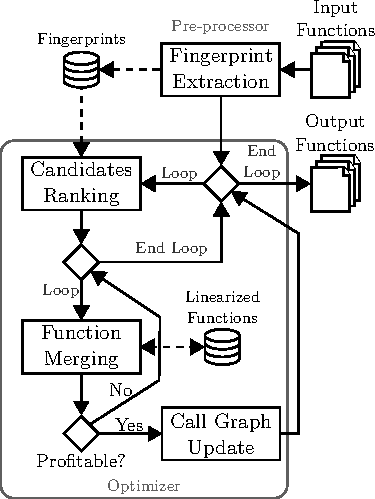
\includegraphics[width=0.7\linewidth]{src/merging-optimisation/figs/func-merge-opt-arch.pdf}
  \caption{Overview of our exploration framework.}
  \label{fig:func-merge-opt-arch}
\end{figure}

The proposed framework is based on a light-weight ranking infrastructure that uses a \textit{fingerprint} of the functions to evaluate
their similarity. It starts by precomputing and caching fingerprints for all functions. The purpose of fingerprints is to make it easy
to discard unpromising pairs of functions so that we perform the more expensive evaluation only on the most promising pairs.
To this end, the fingerprint consists of: $(1)$ a map of instruction opcodes to their frequency in the function; $(2)$ the set of types
manipulated by the function. While functions can have several thousands of instructions, an IR usually has just a few tens of opcodes,
e.g., the LLVM IR has only about 64 different opcodes. This means that the fingerprint needs to store just a small integer array of the
opcode frequencies and a set of types, which allows for an efficient similarity comparison.

By comparing the opcode frequencies of two functions, we are able to estimate
the best case merge, which would happen if all instructions with the same opcode could match.
This is a very optimistic estimation. It would be possible only if instruction types and order
did not matter. We refine it further by estimating another best case merge, this time based
on type frequencies, which would happen if all instructions with the same data type could match.


%This assumption provides an upper bound on the actual number of matches, since
%it may be affected by the instruction types and the order they appear in the
%linearised functions.
%As a way to refine this estimate, we weight this upper bound by the Jaccard
%similarity coefficient~\cite{jaccard} of the sets of types, i.e., a
%type-similarity ratio between the two functions.
%Formally, let $T_1$ and $T_2$ be the set of types of the functions $f_1$ and
%$f_2$, respectively.
%In order to refine this upper-bound estimate, we also compare the type frequencies
%of the two functions, this time assuming that all instructions with the same
%data type would always result in a match.
Therefore, the upper-bound reduction, computed as a ratio, can be generally defined as
%\[
%   U\!B(f_1,f_2) = \frac{\sum\limits_{op \in Ops} \min\{freq(op,f_1),freq(op,f_2)\}}{\sum\limits_{op \in Ops} freq(op,f_1)+freq(op,f_2)}
%\]
\[
   U\!B(f_1,f_2, K) = \frac{\sum\limits_{k \in K} \min\{freq(k,f_1),freq(k,f_2)\}}{\sum\limits_{k \in K} freq(k,f_1)+freq(k,f_2)}
\]
where $U\!B(f_1,f_2, Opcodes)$ computes the opcode-based upper bound and
$U\!B(f_1,f_2, Types)$ computes the type-based upper bound.
The final estimate selects the minimum upper bound between the two, i.e.,
\[
%     s(f_1,f_2) = U\!B(f_1,f_2) \frac{|T_1 \cap T_2|}{|T_1 \cup T_2|}.
     s(f_1,f_2) = \min\{U\!B(f_1,f_2, Opcodes), U\!B(f_1,f_2, Types)\}
\]
This estimate results in a value in the range $[0,0.5]$,
which encodes a description that favors maximizing both the opcode and type
similarities, while also minimizing their respective differences.
Identical functions will always result in the maximum value of $0.5$.

For each function $f_1$, we use a priority queue to rank the topmost
similar candidates based on their similarity, defined by $s(f_1,f_2)$, for all
other functions $f_2$.
We use an exploration threshold to limit how many top candidates we will
evaluate for any given function.
We then perform this candidate exploration in a greedy fashion, terminating after
finding the first candidate that results in a profitable merge and committing that
merge operation.

\begin{figure}[t!]
  \centering
  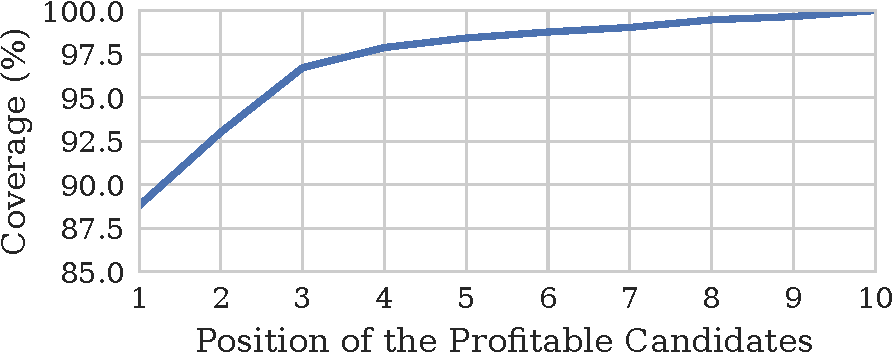
\includegraphics[width=0.8\linewidth]{src/merging-optimisation/figs/average-cdf-exploration-threshold.pdf}
  \caption{Average CDF for the position of the profitable candidate and the percentage of merged operations covered.
           %Average CDF for the exploration threshold and the percentage of merged operations covered.
           89\% of the merge operations happen with the topmost candidate.}
           %A merge operation happens with the topmost candidate in about 89\% of the cases.}
  \label{fig:average-cdf-exploration-threshold}
\end{figure}

Ideally, profitable candidates will be as close to the top of the rank as
possible.
Figure~\ref{fig:average-cdf-exploration-threshold} shows the cumulative
distribution of the position of the profitable candidates in a top 10 rank.
It shows that about 89\% of the merge operations occurred with the topmost
candidate, while the top 5 cover over 98\% of the profitable candidates.
These results suggest that fingerprint similarity is able to
accurately capture the real function similarity, while reducing the exploration
cost by orders of magnitudes, depending on the actual number and size of
the functions.

When a profitable candidate is found, we first replace the body of the two
original functions to a single call to the merged function.
Afterwards, if the original functions can be completely removed, we update the
call graph, replacing the calls to the original functions by calls to the
merged function.
Finally, the new function is added to the optimisation working list.
Because of this feedback loop, merge operations can also be performed on
functions that resulted from previous merge operations.

\subsection{Link-Time Optimisation}

There are different ways of applying this optimisation, with different trade-offs.
We can apply our optimisation on a per compilation-unit basis, which usually
results in lower compilation-time overheads because only a small part of the
whole program is being considered at each moment.
However, this also limits the optimisation opportunities, since only pairs of
functions within the same translation unit would be merged.

On the other hand, our optimisation can also be applied in the whole program,
for example, during link-time optimisation (LTO).
Optimizing the whole program is beneficial for the simple fact that the
optimisation will have more functions at its disposal.
It allows us to merge functions across modules.

\begin{figure}[h]
  \centering
  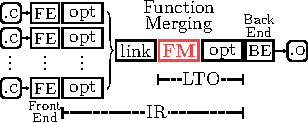
\includegraphics[width=0.7\linewidth]{src/merging-optimisation/figs/opt-pipeline.pdf}
  \caption{In our experiments we use a compilation pipeline with a monolithic link-time optimisation (LTO).}
  \label{fig:opt-pipeline}
\end{figure}


In addition to the benefit of being able to merge more functions, when optimizing
the whole program, we can also be more aggressive when removing the original functions,
since we know that there will be no external reference to them.
However, if the optimisation is applied per translation unit, then extra
conditions must be guaranteed, e.g., the function must be explicitly defined
as internal or private to the translation unit.
